\chapter{基于对比学习的多项选择长文本阅读理解}
多项选择阅读理解是一种通过阅读并理解一篇给定文章和问题,从多个备选答案中选出最合适答案的任务。
近期的研究致力于捕获文章、问题和选项三元组之间的联系,但由于文本长度过长,模型难以重点关注备选答案之间的联系,导致在面临复杂的多项选择问题时,最近的方法往往会将干扰选项误判为正确答案。
为了解决这一问题,本章提出了一种基于对比学习和样本内注意力的模型CoLISA(Contrastive Learning and In-Sample Attention),该模型通过对比学习和样本内注意力机制,相对精准地剔除干扰选项。
特别地,CoLISA采用对比学习来获取蕴含其他选项信息的选项表示,并应用样本内注意力机制,使得多个选项之间产生联系。
实验结果表明,CoLISA在正确与错误选项之间的联系花费了更多注意力,能够识别选项之间的差异,并在QuALITY数据集上实现了SOTA(state-of-the-art)的性能。


\section{引言}
机器阅读理解(Machine Reading Comprehension, MRC)是一种通过对给定文档进行推理,要求模型回答指定问题的任务。
作为MRC任务的一种变体,多项选择阅读理解(Multi-choice Reading Comprehension, MC-RC)主要针对在给定文章的情况下,从多个备选答案中选出最合适的答案来回答问题。
MC-RC要求模型在阅读并理解参考文章的前提下,判断每个备选答案的正确性。

在MC-RC领域,现有的研究通常集中于解决文章和备选答案之间的差异问题,以解决给定问题\cite{ran2019option,zhang2020dcmn+}。
这些模型通常会对每个选项进行独立编码。
然而,这种方法会限制模型的推理能力,因为对于某个问题,每个选项并不能直观地与其他选项进行交互。
此外,在某些真实情况下,某些备选答案在字面上或语义上与正确答案非常相似,这使得仅仅判断单个选项的正确性变得更加困难。
目前已有的方法往往无法处理这些情况。
因此,本章认为需要采用更精细的方法来处理这些所谓的干扰项与正确答案之间的关系。
表~\ref{tab:4-1}~具体描述了QuALITY\cite{pang2021quality}中一个关于难以辨别的干扰项的实例\footnote{QuALITY中也存在输入文章长度超过模型限制的情况,本章也会在后续讨论这个问题。}。
参考例子中的整篇文章,可以认为正确答案$O_2$(表中红色部分)和干扰选项$O_1$(表中蓝色部分)可以认定都是接近于正确答案的。
为了根据给定问题选出最合适的答案,模型需要找到正确答案和干扰选项表示之间的差异。

\begin{table}[htbp]
    \centering
    \begin{tabular}{p{420pt}}
    \hline
    {\bfseries 文章:} \\
    (...) I'm sure that `justifiable yearnings for territorial self-realization' would be more appropriate to the situation (...) (Over 4,000 words) \\
    <译文:(...) 我确信“对领土自我实现的正当渴望”可能更适用于这种情况 (...) > \\
    \hline
    {\bfseries 问题:} \\
    According to Retief what would happen if the Corps did not get involved in the dispute between the Boyars and the Aga Kagans? \\
    <译文:如果Corps不介入Boyars和Aga Kagans的争端,根据Retief的说法会发生什么? > \\
    \hline
    {\bfseries 选项:} \\
    $O_1$: \textcolor[rgb]{0.4,0.7,0.9}{The Aga Kagans would enslave the Boyars} \\
    <译文:Aga Kagans会奴役Boyars> \\
    $O_2$: \textcolor[rgb]{1,0.4,0.3}{The Boyars and the Aga Kagans would go to war} \\
    <译文:Boyars和Aga Kagans会引发战争 > \\
    $O_3$: The Aga Kagans would leave Flamme to find a better planet \\
    <译文:Aga Kagans会离开Flamme,找到更好的星球> \\
    \textbf{$O_4$}: The Boyars would create a treaty with the Aga Kagans without the Corps' approval \\
    <译文:Boyars会与Aga Kagans签订条约,而不需要得到Corps的批准> \\
    \hline
    \end{tabular}
    \caption{\label{tab:4-1}
    QuALITY中的例子。
    }
\end{table}


人类总是需要通过仔细比较各个选项之间的差异,来排除看上去正确的错误选项,从而回答阅读理解-多项选择问题(MC-RC问题)\cite{daniel2017thinking}。
受到该流程的启发,本章提出了一个基于对比学习和样本内注意力(CoLISA)的架构,它包含两个主要的特点。
首先,由于应用了两次不同的dropout掩码,得到两个有着轻微差异的表示。
也就是说,对于同一个输入,会有两组输出值,每一组都包含了一个正确答案和若干个错误选项。
CoLISA主要通过对比学习的方式,将两个正确选项的表示拉近,然后把正确答案与干扰选项之间的表示推远;
因此,该模型可以学习到更有效的文本表示。
此外,自注意力机制\cite{vaswani2017attention}也应用在了特定样本中的多个选项之间,在选项之间共享彼此的信息。
因此,模型借助多个备选答案之间的自注意力交互的方式,学习到了倾向于选择正确答案的能力。
本章还在两个MC-RC数据集QuALITY\cite{pang2021quality}和RACE\cite{lai2017race}上进行了实验。
实验结果表明,CoLISA的性能表现显著超过其他现有方法。

本章的研究贡献可以概括如下:
\begin{itemize}
    \item[$\bullet$] 引入对比学习方法,以区分多项选择长文本阅读理解任务中正确答案和干扰选项之间的差异。该方法通过赋予干扰选项更多的权重,从而使其获得更多的注意力。
    \item[$\bullet$] 针对一个特定的例子,将样本内注意力机制应用于多个选项之间,促进它们之间的互动。
    \item[$\bullet$] 本章提出的CoLISA方法在QuALITY上实现了SOTA的性能,并在RACE上相对于其他基线模型实现了显著的提升。
\end{itemize}


\section{基于对比学习的多项选择长文本阅读理解}
给定一篇参考文本,一个目标问题,还有一些备选答案,多项选择阅读理解(multi-choice reading comprehension, MC-RC)任务是指将其中一个选项预测为最终答案。
形式上来说,将一篇文章定义为$p=[s^p_1, s^p_2, ..., s^p_n]$,其中$s^p_i=[w^s_1, w^s_2, ..., w^s_l]$表示$p$中第$i$个句子,$w^s_j$表示$s^p_i$中的第$j$个词。
问题可以定义为$q=[w^q_1, w^q_2, ..., w^q_t]$,其中$w^q_i$表示$q$中的第$i$个词。
选项集合可以定义为$O=[o_1, o_2, ..., o_r]$,其中$o_i=[w^o_1, w^o_2, ..., w^o_k]$表示第$i$个选项,$w^o_k$表示$o_i$中第$k$个词。
MC-RC的目标是最大化所预测选项的概率:
\begin{equation}
    a = \argmax_i(\mathcal P(o_i|p,q))
\end{equation}

当$p$的长度超过编码器的最大输入长度时,本章的做法是通过检索与问题和备选答案相关的句子,将长文本压缩成篇幅较短的文本。
较短文本表示为$c=[s^c_1, s^c_2, ..., s^c_m]$,其中$s^c_i=[w^s_1, w^s_2, ..., w^s_l]$表示$c$中的第$i$个句子,$w^s_j$表示$s^c_i$中的第$i$个句子。

\subsection{总体架构}
如图~\ref{fig:4-1}~所示,本章提出了一种新颖的MC-RC框架,它充分运用了对比学习和样本内注意力(Contrastive Learning and In-Sample Attention, CoLISA),主要由两部分组成:
首先是基于DPR(Dense Passage Retrieval,稠密检索)的检索器,在一篇很长的文章中,根据对给定问题和对应的过个备选答案之间的相关性,筛选出相关的句子,以此来根据原文的原始顺序来构建一段新的文本;
另外,CoLISA阅读器需要根据给定问题和上下文中,从若干选答案中预测出最终答案。
CoLISA阅读器由两部分组成。
第一部分是样本内注意力(In-Sample Attention, ISA)机制,换句话说,引入一个加入了多头自注意力机制并针对长序列的网络,来增强特定样本中多个选项之间的交互。
第二部分是对比学习(Contrastive Learning,CoL)以及一个干扰因子(Distractive Factor,DiF),来表示由上下文、问题和备选答案组合而成的序列。

% 模型图
\begin{figure}[htbp]
    \centering
    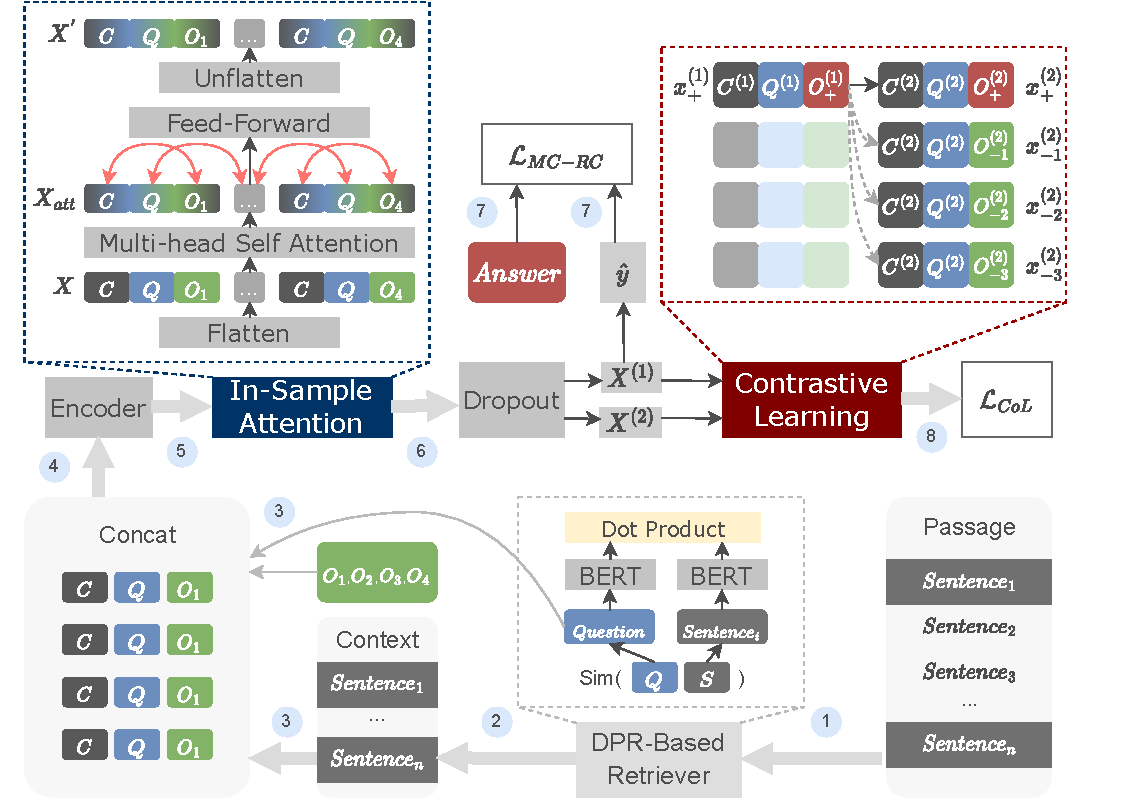
\includegraphics [width=1.0\textwidth] {figure/4-1.pdf}
    % \caption{The architecture of our model CoLISA. (1) A long passage is fed into the DPR-based retriever, (2) then comes out a shorter context, (3) together with a related question and multiple options in our dataset, they are (4) preprocessed and combined into four different sequences (in our dataset there are four options for each question), after going through the inherent (5) embedding and (6) encoder, these four sequences are represented as (7) vector representations, (8) followed by an ISA module listed on the right top of the figure, the sequences are flattened to a combined one, with multi-head self-attention across each token within the extended sequence, then the sequence roll back to the initial dimension, (9) the updated vectors are fed into a dropout twice to come out into two outputs, (10) one for calculating the cross-entropy loss (11) meanwhile both of them need feeding to a CoL module illustrated on the left top of the figure, to calculate a contrastive learning loss finally.}
    \caption{CoLISA的基本架构。} % Our proposed contrastive learning method and in-sample attention mechanism are highlighted boldly in dark red and dark blue rectangles, respectively.
    \label{fig:4-1}
\end{figure}


\subsection{基于DPR的检索器}
为了从一篇长文本中筛选出相关的句子,本节首先采用基于DRP(Dense Passage Retrieval,稠密检索)的句子检索器。
该检索器常用于隐式语义编码\cite{karpukhin2020dense}。
值得注意的是,DPR提供了两个不同的编码器,用于预训练抽取不同种类的句子,本节使用相应的DPR编码器以确保检索到的句子具有多样性。
上下文编码器$E_S$将参考文章$p$中的所有句子$s$编码为$d$维向量。
类似地,查询编码器$E_R$将问题$q$和选项集合$O$编码为$d$维向量,作为两种不同的检索查询$r$。
$s$和$r$的$[CLS]$token的全局表示用于计算它们的负欧几里得距离($L^2$):
\begin{equation}
    -L^2_{dist}(r,s)=-||E_R(r)-E_S(s)||^2
\end{equation}

针对选项查询,本节按照$s$和$r$之间的相关性降序排列,选择前$k$个句子,并考虑到语义连贯性的问题,筛选出这$k$个句子的前一句和后一句。
然而,同一个句子可能会被多次选择,因此需要去重。
最终得到$k$个唯一的句子作为参考上下文。

对于问题查询,首先选择前$n$个句子作为参考上下文\footnote{考虑到预训练语言模型能容纳所抽取的句子的总长度,$k$和$n$需要设定为合适的值,这里在所有实验中将$k$设为2,$n$设为1。}。
由于来源于选项的证据相比于来源于问题的证据更合适,所以本节不采集前一句和后一句。
同样,需要通过去重来确保所有抽取句子的唯一性。

在选出最合适的句子后,再根据原文顺序将这些句子进行排序,然后将它们拼接成一段参考上下文$c$。
算法~\ref{alg:4-2}~详细阐述了抽取的过程。

% \begin{algorithm}\small
%   \KwIn{Passage $p=[s_1, s_2, ..., s_n]$, Question $q$, Options $O=[o_1, o_2, ..., o_m]$}
%   \KwOut{Context}
%   \eIf{Input (x) belongs to p}{
%     $E_x$ = ContextEncoder($x$)\;
%     }{
%     $E_x$ = QuestionEncoder($x$)\;
%     % $E_o$ = QuestionEncoder($o$)\;
%     }
%   \For{$o_i$ in $O$}{
%     \For{$s_j$ in $p$}{
%       sim($o_i$, $s_j$) = -L^2_{dist}($E_{o_i}$, $E_{s_j}$)
%       }
%     Select: Top-k relevant sentences $s_{i_1}, s_{i_2}, ..., s_{i_k}$\;
% 	Select: Their previous and next sentences $s_{i_1}^{prev}, s_{i_1}^{next}, ..., s_{i_k}^{prev}, s_{i_k}^{next}$\;
% 	Context $\gets$ Selected sentences\;
% 	}
%   \For{$s_j$ in $p$}{
%     sim($q$, $s_j$) = -L^2_{dist}($E_q$, $E_{s_j}$)
% 	}
%   Select: Top-n relevant sentences $s_{j_1}, s_{j_2}, ..., s_{j_n}$\;
%   Context $\gets$ Selected sentences\;
%   Context.unique().sort().to\_str()\;
%   \caption{\label{alg:algorithm}The Extracting Algorithm}
% \end{algorithm}


\begin{algorithm}\small
  % \KwIn{Passage $p=[s_1, s_2, ..., s_n]$, Question $q$, Options $O=[o_1, o_2, ..., o_m]$}
  % \KwOut{Context}
  % \eIf{Input (x) belongs to p}{
  %   $E_x$ = ContextEncoder($x$)\;
  %   }{
  %   $E_x$ = QuestionEncoder($x$)\;
  %   % $E_o$ = QuestionEncoder($o$)\;
  %   }
  % \For{$o_i$ in $O$}{
  %   \For{$s_j$ in $p$}{
  %     sim($o_i$, $s_j$) = -L^2_{dist}($E_{o_i}$, $E_{s_j}$)
  %     }
  %   Select: Top-k relevant sentences $s_{i_1}, s_{i_2}, ..., s_{i_k}$\;
	% Select: Their previous and next sentences $s_{i_1}^{prev}, s_{i_1}^{next}, ..., s_{i_k}^{prev}, s_{i_k}^{next}$\;
	% Context $\gets$ Selected sentences\;
	% }
  % \For{$s_j$ in $p$}{
  %   sim($q$, $s_j$) = -L^2_{dist}($E_q$, $E_{s_j}$)
	% }
  % Select: Top-n relevant sentences $s_{j_1}, s_{j_2}, ..., s_{j_n}$\;
  % Context $\gets$ Selected sentences\;
  % Context.unique().sort().to\_str()\;
  \caption{\label{alg:algorithm}The Extracting Algorithm}
\end{algorithm}


\subsection{样本内的自注意力机制}
在进行编码$q$和$o_i$时,针对同一个问题,每个备选答案的编码都是相互独立的,这导致在计算注意力时可能会出现注意力缺失的问题。
为了解决这个问题,本章借鉴了人类回答多项选择问题的方式,即通过同时比较多个选项来排除干扰项,最终决定选择哪个选项。
基于这种思路,本章提出了一种样本内注意力(In-Sample Attention)机制,以增强不同选项表示之间的交互作用。

通常,每个备选答案$o_i$先和它对应的上下文$c$以及问题$q$进行拼接,构成一个三元组$x_i=[c;q;o_i]$。
本章通过将每个$x_i$依次喂入预训练编码器中,从而得到一系列完整的序列表示。
为了建模多个选项$o_i$之间的联系,本章提出的ISA模块首先收集到所有与相同问题$q$对应的$x_i$,对它们进行拼接,构建一个单独的序列$X=[x_1;x_2;...;x_n]$。
然后,计算$X$的自注意力表示,来学习多个选项之间的远程依赖。
具体来说,利用平凡的自注意力机制的架构,同时将序列$X$分解为三个矩阵$Q$,$K$,$V$。
输出的自注意力矩阵可以计算为:
\begin{equation}
    SA(Q,K,V)=softmax(\frac {QK^T}{\sqrt{d_k}})V
\end{equation}
其中$d_k$是一个缩放因子,它表示$K$的维度,以防引起梯度消失现象\cite{vaswani2017attention}。
更进一步,多头注意力机制被引入到ISA中,从不同的向量维度来更加综合性的表示$X$。
多头自注意力的流程可以定义为:
\begin{align}
    & head_i = SA(QW^Q_i,KW^K_i,VW^V_i) \\
    & H = Concat(head_1,...,head_h) \\
    & MSA(Q,K,V) = HW^O
\end{align}
其中$h$表示各个平行注意力头的数量,$W^Q_i,W^K_i,W^V_i,W^O$是注意力参数矩阵。
这里还将多头自注意力的向量表示记为$X_{att}$。
如图~\ref{fig:4-1}~中的ISA机制所描述的,作用在拼接后的序列$X$的注意力机制通过计算选项之间的表示$X_{att}$,实现彼此之间的交互。

此外,为了避免多头自注意力输出的塌陷\cite{vaswani2017attention,sukhbaatar2019augmenting},多头自注意力机制后面还增加了一个全连接网络:
\begin{equation}
    X_{ffn}=FFN(X_{att})
\end{equation}
这里使用了GeLU\cite{hendrycks2016gaussian}函数作为激活函数。
最终,$X_{fnn}$需要根据多个输入三元组$x_i$的维度拆解为多个表示。
输出三元组的结合记为$X^{'}$。

\subsection{面向备选答案交互的对比学习方法}
为了推动CoLISA在明确区分正确答案和干扰选项表示之间的差异方面的表现,本节引入了对比学习(Contrastive Learning,CoL)模块。
受通用对比学习框架\cite{gao2021simcse}的启发,CoL模块旨在通过将同一样本内的所有表示均匀分布在特定的向量空间上,促进两个正向三元组表示之间的变得更加接近。

在上一节介绍的ISA模块之后,具有交互注意力的输入向量$X^{'}$通过dropout层进行传递,并进行两次相同的操作,以针对每个输入生成两个略有差异的编码表示,分别记为$X^{(1)}$和$X^{(2)}$。

之后,先要计算MC-RC任务中在目标标签$y$和输出$X^{(1)}$之间的交叉熵损失。
具体来说,通过一层全连接神经网络可以将$X^{(1)}$转换为预测输出$\hat y$,它的维度与标签$y$相同。
损失函数定义如下:
\begin{equation}
    \begin{split}
    \mathcal L_{MC-RC}=& -\frac{1}{N}\Sigma^N_{i=1}(y^{(i)}\log\hat y^{(i)}+(1-y^{(i)})\log(1-\hat y^{(i)}))
    \end{split}
\end{equation}
注意到来自同一样本的输出$X^{(1)}$和$X^{(2)}$均由相同数量的三元组$x_i$组成,其中包含一个正确答案的三元组以及其余包含错误答案的三元组。
因此,对于每个输入样本的两个输出结果,对比损失可以被定义为负对数似然函数的平均值。
具体而言,对于其中一个输出$X^{(1)}$,本节将包含正确答案的三元组作为锚点,并移除包含错误选项的三元组。
对于另一个输出$X^{(2)}$,所有三元组均被保留,其中包含正确选项的三元组视为正例,而其他三元组则被视为负例。
每个损失项均能够区分正例和负例之间的差异。

CoL的损失函数定义如下:
\begin{equation}
    \mathcal L_{CoL}=-\frac{1}{N}\Sigma^N_{j=1}\log \frac{e^{sim(x^{(1)}_+,x^{(2)}_+)/ \tau}}{\Sigma^S_{i=1} e^{sim(x^{(1)}_+,x^{(2)}_i)/ \tau}}
\end{equation}
其中$x^{(1)}_+$是$X^{(1)}$中包含正确答案的三元组的编码表示,而$x^{(2)}_i$是$X^{(2)}$中所有三元组的表示,$X^{(2)}$中的$x^{(2)}_+$是正例样本,$\tau$是可配置的超参数,温度系数。
$sim(\cdot)$是一种相似度指标(本章中所有的实验都是使用余弦相似度函数),$S$代表了每个样本中三元组的数目,$N$代表了batch的大小。
聚合后的对比损失$\mathcal L_{CoL}$主要通过在每个batch中的所有样本取平均获得。

\textbf{干扰因子。}
基于样本中不同的干扰项会对模型造成不同程度的干扰,本节还将一个对比因子(Distractive Factor, DiF)引入到了CoLISA模型,具体来说,将DiF结合到对比学习的过程当中。
QuALITY的数据标注人员针对每个问题的所有错误选项中,把误导他们最严重的的那个标记为强干扰项。
因此,本节中通过构建一组置信因子,根据每个选项对应的标注分数,来代表它们对$\mathcal L_{CoL}$的贡献度。
本节中枚举了对每个选项的标注票数来构建DiF $\Theta=[\theta_1, \theta_2, ..., \theta_n]$,其中$n$是备选答案的数量。
然后再用一个softmax函数来帮助缩放$\Theta$,从而更明显的区分每个$\theta_i$。
每个$\theta_i$被修正为如下的形式:
\begin{equation}
    \theta_i=\frac{e^{\theta_i}}{\Sigma^n_i e^{\theta_i}}
\end{equation}
幂运算可以清晰的却分$n$个系数$\theta_i$。
当计算对比损失的时候,$\theta_i$乘上了它对应选项的相似度的值,来衡量正确答案和干扰答案的差距。
$\theta_i$的值越大,对对应选项贡献的损失就越多。
经过上述分析,对比损失函数可以改进为如下:
\begin{equation}
    \mathcal L_{CoL}=-\frac{1}{N}\Sigma^N_{j=1}log \frac{\theta_+e^{sim(x^{(1)}_+,x^{(2)}_+)/ \tau}}{\Sigma^S_{i=1} \theta_ie^{sim(x^{(1)}_+,x^{(2)}_i)/ \tau}}
\end{equation}
其中$\theta_+$和$\theta_i$分别对应样本中的正例以及第$i$个选项。
最终的损失函数可以表示为:
\begin{equation}
    \mathcal L=\alpha \cdot \mathcal L_{MC-RC}+(1-\alpha) \cdot \mathcal L_{CoL}
\end{equation}
其中$\alpha \in[0,1]$是一个平衡系数。


\section{实验及结果分析}
本节首先详细描述了实验的设置,并在此基础上呈现了实验结果。
接着,本节对实验结果进行了进一步的对比和分析,特别是与其他现有模型进行了比较。
此外,本节还进行了一系列消融实验,以验证CoLISA模型的有效性和鲁棒性。

\subsection{实验设置}
本节采用了基准数据集QuALITY和RACE,以评估CoLISA模型的效果。
其中,主要实验是在QuALITY数据集上进行的\footnote{基于DPR的检索器在QuALITY数据集中对于长文本输入的检索是可行的。此外,最强干扰项仅在QuALITY数据集中有标注,因此,大部分实验均在该数据集上完成。}。同时,本节也报告了在RACE数据集上的其他实验结果。

\begin{itemize}
    \item QuALITY~\cite{pang2021quality}。这是一个多项选择阅读理解(MC-RC)数据集,其每篇文章的平均长度约为5000个token。该数据集的一个显著特征是一些干扰选项会对模型的认知能力造成负面影响。因此,如果不依靠摘要或文本片段,略读和简单的搜索已经不足以让模型持续表现出优异的性能。该数据集的文本主要采集自科幻小说和杂志,并由标注人员进行阅读和评估。
    \item RACE~\cite{lai2017race}。由于QuALITY只由6,737条源数据构成,难以全面评估实验结果,因此实验中还使用了另一个大规模MC-RC数据集RACE来验证模型的性能。RACE从中国的中考和高考英语阅读理解试题中收集。大多数问题需要推理,并且文本涉及的领域是多样的,从新闻、故事到广告,这使得数据集更具挑战性。
\end{itemize}

本章主要研究针对QuALITY\cite{pang2021quality}和RACE\cite{lai2017race}两大数据集的多项选择问答任务。
为了评估模型的性能,本章采用准确率(Accuracy, ACC)作为主要的评估指标,用以衡量模型在回答问题时的正确率。
由于两个数据集中存在不同难度的文本,因此本章的实验也分别考虑了QuALITY数据集中全部/困难子集的$acc$以及RACE数据集中中考/高考子集\footnote{在QuALITY数据集中,源数据根据问题难度分为全部和困难子集,而在RACE数据集中,中考和高考子集代表了两个水平的入学考试试题。}的$ACC$。
对于基于DPR的检索器,本章采用了与QuALITY数据集中的基线模型相同的方法来减轻检索稀疏性的影响,以便进行公平比较。
具体而言,本章使用了一个问题编码器对查询进行编码,以及一个上下文编码器对文章进行编码。

本节针对CoLISA的阅读器,采用了DeBERTaV3-large模型作为预训练语言模型。
在QuALITY和RACE上的所有实验中,学习率均为1e-5,热身率为0.1。
此外,Dropout比例保持默认的0.1,激活函数采用了GeLU\cite{hendrycks2016gaussian}。
所有实现均使用16的batch尺寸和512个token的最大长度。
在QuALITY上进行了20轮的模型微调,在RACE上进行了3轮的微调。

为进行对比学习,由于实验开销的原因,本文在DeBERTaV3-base和RoBERTa-base模型上调整了温度系数$\tau$。
经过调参,基础模型上最优的$\tau$值为0.1,该值直接应用于大模型中。
同时,交叉熵损失和对比损失分别分配一半到最终的综合损失中。
此外,先前提到的干扰因子仅仅应用于QuALITY的实验中,因为RACE数据集没有对所有选项进行干扰程度标注。

所有实验都在一张Tesla V100-32GB的GPU上进行训练,Apex中的fp16精度模式也用于加速训练过程。

虽然在QuALITY上有许多方法可以进行尝试,但本章仅选取了两个典型的基线模型。

\begin{itemize}
    \item Longformer~\cite{beltagy2020longformer}。
        该预训练语言模型结合了滑动窗口局部注意力和全局注意力机制,来编码较长的文本序列。
        Longformer支持最多达到4,096长度的输入序列。
        实验对比过程中采取了Longformer作为其中一个基线模型,因为它包含了需要回答QuALITY样本中大部分的文本。
    \item DPR \& DeBERTaV3~\cite{karpukhin2020dense,he2021debertav3}。
        该管道架构由一个检索器和一个阅读器组成。
        基于DPR的检索器用于在一篇文章中针对指定问题抽取最相关的上下文。
        被选取的上下文作为输入的一部分,将被喂给后续的模块。
        最后,一个用于MC-RC标准的DeBERTa-V3模型将会抉择出正确的答案选项。
\end{itemize}

\subsection{实验结果和分析}
本节对CoLISA模型与两个QuALITY上强力的基线模型进行比较,以及RACE上三个预训练语言模型进行比较进行分析。
总体而言,表~\ref{tab:4-3}~所示的结果表明\footnote{本节在QuALITY数据集上进行了DPR和DeBERTaV3架构基线的重新实现(标有*),表现明显优于QuALITY原文中的记录(53.6/47.4)。DeBERTaV3-large的结果也是如此。而其他基线结果则来自相关研究或相关排行榜。在RACE数据集上的实验不需要基于DPR的检索器和干扰因素。在训练过程中,QuALITY数据集中的模型是中间经过RACE数据集训练并在QuALITY上进行微调的。},CoLISA模型优于其他所有模型。
其中,Longformer模型的性能不佳,这说明Longformer模型在处理冗长的源文本时无法准确定位关键信息。
这可能是由于长文本预训练语言模型需要更多的训练数据,而QuALITY提供的训练数据十分有限所致。
此外,QuALITY中文本的长度仍超过了Longformer模型的最大编码长度限制,这可能会导致关键信息的丢失。
相比之下,DPR和DeBERTaV3架构由于其自身的抽取策略,性能表现更为突出。
与之前提到的两个基线模型相比,CoLISA模型学习到了更有效的上下文表示方法,并通过引入的对比学习(CoL)策略,更加准确地识别多个备选答案之间的差异。
同时,将ISA机制引入DeBERTaV3编码器之后,可以持续增强模型的性能表现。
这种尝试意味着,用ISA风格的方式在多个选项之间进行内部交互,将进一步捕捉到所有备选答案之间的差异关系。

\begin{table}\scriptsize
    \centering
    \begin{tabular}{ll|ll|ll|ll}
    \hline
    {\bfseries Model} & {\bfseries Acc} & {\bfseries Model} & {\bfseries Acc} & {\bfseries Model} & {\bfseries Acc} & {\bfseries Model} & {\bfseries Acc} \\
    \hline
    Baseline & 56.7 & Baseline & 56.7 & Baseline & 56.7 & Baseline & 39.6 \\
    \hline
    CoL & {\bfseries 60.1} & CoL & 60.1 & CoL & 60.1 & CoL & {\bfseries 40.8} \\
    \hline
    $\ $ question query & 58.9 & $\ $ w/ DiF & {\bfseries 60.9} & $\ $ w/ self-attention & 60.4 & $\ $ in-batch negatives & 37.1 \\
    $\ $ in-batch negatives & 59.4 & $\ $ KL Loss & 57.0 & $\ \ $ context masked & 60.4 & \\
    & & & & $\ $ w/ transformer & {\bfseries 61.0} & & \\
    & & & & $\ $ w/ transformer*2 & 60.8 & & \\
    & & & & $\ $ w/ modified transformer & 58.9 & & \\
    \hline
    \end{tabular}
    \caption{\label{tab:4-3}
    Ablation study on contrastive learning module, distractive factor, and in-sample attention mechanism on the development set of QuALITY.
    }
\end{table}


\subsection{消融实验}
\textbf{对比学习。}
为了有效评估CoL模块对整个模型表现的影响,本节进行了一个消融实验,具体如表~\ref{tab:4-4}~中的第一列所示。
首先,在抛弃ISA模块的情况下,可以评估仅使用对比学习方法对模型整体性能的影响。
实验结果表明,相比于基线模型(即表中前三列DPR \& DeBERTaV3-large的架构),单独使用CoL组件的方法显著提升了模型性能。

\begin{table}\scriptsize
    \centering
    \begin{tabular}{ll|ll|ll|ll}
    \hline
    {\bfseries Model} & {\bfseries Acc} & {\bfseries Model} & {\bfseries Acc} & {\bfseries Model} & {\bfseries Acc} & {\bfseries Model} & {\bfseries Acc} \\
    \hline
    Baseline & 56.7 & Baseline & 56.7 & Baseline & 56.7 & Baseline & 39.6 \\
    \hline
    CoL & {\bfseries 60.1} & CoL & 60.1 & CoL & 60.1 & CoL & {\bfseries 40.8} \\
    \hline
    $\ $ question query & 58.9 & $\ $ w/ DiF & {\bfseries 60.9} & $\ $ w/ self-attention & 60.4 & $\ $ in-batch negatives & 37.1 \\
    $\ $ in-batch negatives & 59.4 & $\ $ KL Loss & 57.0 & $\ \ $ context masked & 60.4 & \\
    & & & & $\ $ w/ transformer & {\bfseries 61.0} & & \\
    & & & & $\ $ w/ transformer*2 & 60.8 & & \\
    & & & & $\ $ w/ modified transformer & 58.9 & & \\
    \hline
    \end{tabular}
    \caption{\label{tab:4-4}
    Ablation study on contrastive learning module, distractive factor, and in-sample attention mechanism on the development set of QuALITY.
    }
\end{table}


对于基于DPR的检索器,CoL组件将问题和多个备选答案都作为查询词,从参考文章中抽取上下文。
相比之下,仅使用问题作为查询词会导致性能大幅下降。
这一结果的解释是,CoL方法主要针对于将正确答案和干扰选项进行区分,从而更好地抽取与问题/备选答案相关的证据文本。

通过使用标准的dropout两次,可以得到两个不同的语义文本的表示。
在对比学习的过程中,每一个表示分别包含了一个正例。
在收集负例的时候,先前的工作会将同一个batch中剩余的样本视为负例,通常称之为batch内的负例\cite{gao2021simcse}。
本节也测试了一下batch内负例的方法。
遵循这种方法,实验结果揭示,将构建负例的方法从样本内部改为batch内部,会导致性能下跌\footnote{事实上,基础模型上的性能远远低于表格中列出的,当把相同的实验从大模型迁移到基础模型时,会表现出更差的性能。结果列在了表~\ref{tab:4-4}~的最后一列中。性能从40.8疯狂跌到37.1。这里的基线模型是RoBERTa-base。对于大模型,由于机器设备的限制,实验中不得不使用一个较小的batch尺寸。因此,在大模型上无论是batch内的方法还是样本内的方法,都不能展示出巨大的差异。}。
在同一个batch内,多个样本之间没有必然的联系,这就违背了将正确答案按和干扰选项推远的目标。

\textbf{干扰因子。}
正如之前所提到的,CoLISA中设计了一个专门针对QuALITY的干扰因子(Distractive Factor, DiF),以强调困惑选项的作用。
表~\ref{tab:4-4}~中的第二列展示了DiF的实现结果。
本节中将DiF $\Theta$与相应选项的相似度进行相乘操作,以体现对干扰项的权重。
实验结果表明,DiF模块显著提高了CoL模块的性能。
一个直观的解释是,DiF迫使干扰选项对比损失贡献更多的数值,从而使模型更倾向于学习如何识别干扰选项。

基于一个假设,每个备选答案成为最终答案的概率分布遵循特定的概率分布。
本节在实验中使用KL散度损失\cite{hershey2007approximating}替换原来的交叉熵损失,这是一种直观的做法。
实验结果表明,KL散度损失的效果与DiF相似。
此外,交叉熵损失对于正确区分每个三元组(即上下文、问题和备选答案)的正确性至关重要。

\textbf{样本内注意力。}
如表~\ref{tab:4-4}~中的第三列所示,本节中还利用了ISA机制的变体来验证它们的有效性。
可以如预期中观察到,当ISA机制是自注意力机制时,实验性能会由于多个三元组之间存在交互而提升。
然后,实验进一步尝试去遮蔽上下文token,这就意味着只有问题与选项彼此之间可以进行注意力交互,并没有上下文信息的参与。
结果性能是维持不变,这表明问题和备选答案之间的注意力交互是关键的步骤。

消融实验也进一步展示了transformer架构优于单独的一层自注意力层。
这是因为,transformer内部的前馈网络保留了大量的参数,来确保注意力输出的传播。
另有一个有趣的现象,如果再配上额外的一层transformer层,会导致模型性能轻微的下降。
本节认为,从RACE和QuALITY上先后微调的checkpoint被继续沿用,扩充了随机初始化的参数,这会加重训练负担。

此外,本节还通过移植编码器内部的注意力机制,修改了基础编码器的内部结构。
整个预训练编码器由$n$层\footnote{对于基础模型,$n$是12;对于大模型,$n$是24。}组合而成,其中每一层共享完全相同的结构:一个多头自注意力子层和一个前馈神经网络子层。
接下来,本节也针对多项选择的交互,尝试在两个子层之间增加了一个额外的注意力层。
注意到,更低的层主要表达浅层的语义,而更高的层主要针对深层语义,实际操作中只在在顶端的4层补充了注意力机制。
这种修改过后的transformer架构直觉上建模了低层次中的序列内交互,以及高层次中的多序列交互。
实验结果表明,修改编码器架构并不是最好的方法,因为这么做并没有完全利用预训练的成果。


\section{本章小结}
本章主要研究多项选择长文本阅读理解的学习方法和注意力机制,旨在解决备选答案中的干扰选项问题。
本章提出的方法CoLISA通过实现多个选项之间的交互,有效地解决了正确答案和干扰选项之间对比的难题。
CoLISA在两个基准数据集上的实验表明,其性能得到了持续的提升。
未来的研究方向可以探索更多与对比学习方法相关的变体。


